\begin{frame}[fragile]{Patching: Revert}
  \begin{figure}
    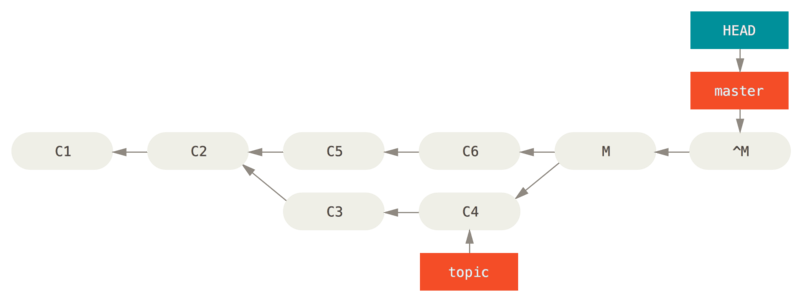
\includegraphics[width=0.8\textwidth]{patching/undomerge-revert}
    \caption{History after revert}
  \end{figure}
  \begin{minted}[
      breaklines,
      frame=single,
      fontsize=\footnotesize
    ]{bash}
git revert -m 1 HEAD
  \end{minted}
  \begin{itemize}
    \footnotesize
    \item The new commit has two parents: C4, C6.
    \item We want to undo all the changes introduced by C4.
    \item The `-m 1` flag indicates to keep all the content from parent 1 (C6).
  \end{itemize}
\end{frame}
